%% Einleitung.tex
%% $Id: einleitung.tex 61 2012-05-03 13:58:03Z bless $
%%

\chapter{Einleitung}
\label{ch:Einleitung}
%% ==============================

In der digitalen Gesellschaft und im Zeitalter des Internets wird es immer wichtiger immer mehr Daten so schnell wie möglich zu speichern.  \textit{Ein Speicher (v. lat.: spicarium Getreidespeicher, aus spica Ähre)[...] ist ein Ort oder eine Einrichtung zum Einlagern von materiellen oder} \textbf{\textit{immateriellen}} \textit{Objekten.}\cite{wiki:Speicher}
\newline
Ein Speichermedium dient also zur kurz- oder langfristigen \glqq \textit{Einlagerung}\grqq{} bzw. \mbox{Erhaltung} von immateriellen Objekten --- oder anders ausgedr"uckt Informationen. 
Es stellt sich die Frage: Was sind Informationen? \newline
Im Laufe der Geschichte wurde der Informationsbegriff immer wieder neu definiert. Für die Informatik ist die Beschreibung nach Claude Elwood Shannon\footnote{Claude Elwood Shannon:* 30. April 1916 in Petoskey, Michigan; \textdagger{} 24. Februar in Melford, Massachusetts gilt als Begr"under der Informationstheorie} relevant. Demnach muss man ein Zeichen als kleinste Informationseinheit und dessen \mbox{statistische} H"aufigkeit in einem Code als Information sehen. 
\newline
Die Information darf nicht mit dem Bedeutungsgehalt verwechselt werden. Eine Information die wenig Sinn ergibt ist einer Information mit großem Sinngehalt gleichwertig. Wichtiger zu betrachten ist die Wahrscheinlichkeit des Auftretens eines Zeichens im vorgegebenen Code. Je geringer diese ist, desto h"oher ist sein \mbox{Informationsgehalt}.
\\
Im wesentlichen werden Informationen aber in Form von Daten auf Speichermedien abgelegt. 
\\Mehrere aufeinanderfolgende Zeichen werden als Zeichenfolge bezeichnet.\cite{hansen:wi1}
\\ 
Daten sind nach ISO 2382 
\glqq \textit{Gebilde aus Zeichen oder kontinuierliche Funktionen, die aufgrund bekannter oder unterstellter Abmachungen Informationen darstellen, vorrangig zum Zweck der Verarbeitung und als deren Ergebnis.}\grqq{}\textbf{TODO:quelle} 
\\
Somit sind nach einer bestimmten Syntax angeordneten Zeichen \textbf{Daten}.

%% ==============================
\section{Zielsetzung der Arbeit}
%% ==============================
\label{ch:Einleitung:sec:Zielsetzung}

Mit dieser Arbeit möchte ich auf grundlegende Prinzipien der Speicherung von Informationen auf verschiedenen Medien, insbesondere in der Informatik eingehen. Sie soll eine "Ubersicht auf M"oglichkeiten der Datenspeicherung f"ur Personal Computer im heutigen Informationsalter schaffen und die grunds"atzliche Funktionsweise der Speichermedien erkl"aren. Auch wenn der Titel \glqq Speicherkomponenten eines PCs\grqq{} ist, wird der Vollst"andigkeit halber trotzdem zum Teil auf "altere Wege Daten zu speichern R"ucksicht genommen. Der Leser sollte nach dem Lesen der Arbeit einen "Uberblick dar"uber haben, welche modernen Methoden es gibt Informationen aufzubewahren. Es werden keine neuen wissenschaftlichen Erkenntnisse vorgestellt, sondern fachliche Informationen zusammengestellt.

%% ==============================
\section{Gliederung der Arbeit}
%% ==============================
\label{ch:Einleitung:sec:Gliederung}

Man unterscheidet zwischen technischer und nichttechnischer Speicherung. Die Speicherung von Informationen ist aber nicht einer Erfindung der Neuzeit. Seit jeher versucht der Mensch Informationen zu bewahren, damit diese nicht in Vergessenheit geraten. 
\\
So geh"oren auch H"ohlenmalereien dazu. Man sch"atzt, dass die "alteste H"ohlenmalerei etwa 40.000 Jahre alt ist. Die Abbildung \ref{fig:hohlenmalerei}  zeigt diese H"ohlenmalerei --- es sind H"ande auf einer Steinwand. Bei dieser sogenannten nichttechnischen Speicherung ben"otigt es ein Tr"agermaterial wie Papier, Pergament, Papyrusrollen oder wie in diesem Beispiel Stein um Informationen zu erhalten. Ein gro"ser Nachteil kann jedoch die sp"atere Entzifferung der \glqq Daten\grqq{} sein, aber immerhin kann man diese sofort auslesen, das hei"st es werden keine zus"atzlichen technischen Ger"ate ben"otigt Informationen zu lesen.

\begin{figure}[ht]
\centering
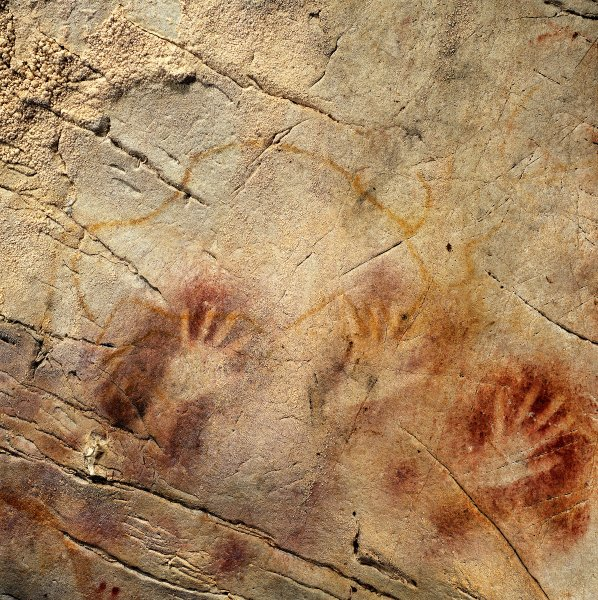
\includegraphics[width=0.7\textwidth]{images/hohlenmalerei.jpeg} 
\caption["alteste bekannte H"ohlenmalerei \cite{fig:hohle}]{"alteste bekannte H"ohlenmalerei}
\label{fig:hohlenmalerei}
\end{figure}


Bei der technischen Speicherung bedarf es einer speziellen Methode um die gew"unschten Daten auszulesen. \\Diese sind nicht sofort per Auge oder mit der Hand erkennbar(vgl. Braille\footnote{Braille: Schrift der Blinden. Die Schrift(verschiedene angeordnete Punkte) wird von Hinten auf Papier gepresst. Diese sind so mit den Fingern ertastbar}). 
%TODO: eingehen auf untere Kapitel(elektronische,magnetische speicherung etc
\\
Die Arbeit ist dementsprechend in diese beiden Teile strukturiert, wobei auf den nichttechnischen Teil nur kurz der Vollst"andigkeit halber eingegangen wird.
Im zweiten Teil ist die Arbeit nach der Zugriffsgeschwindigkeit der einzelnen Speicherkomponenten sortiert. In der Regel sind Komponenten, die intern verbaut sind durch ihren kurzen Weg zur CPU\footnote{Central Processor Unit: Hauptprozessor} und Bauartbedingt schneller.
\\
Dabei wurde sich grob an Abbildung \ref{fig:geschPyr} gehalten. Sie zeigt das Verh"altnis von Kapazit"at zu Zugriffsgeschwindkeit. Desto gr"o"ser die Speicherkapazit"at eines Mediums ist, umso langsamer ist dessen Zugriffsgeschwindkeit. 
\begin{figure}[ht]
\centering
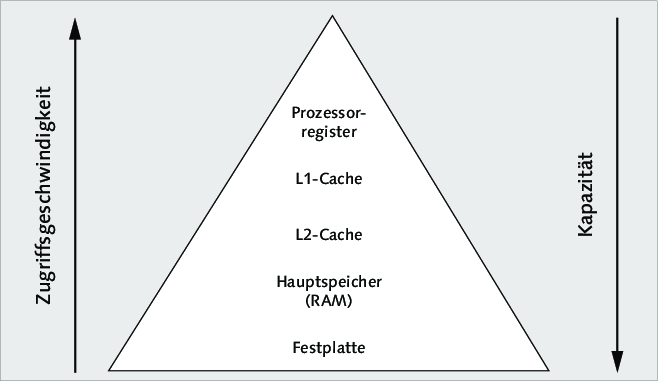
\includegraphics[width=0.7\textwidth]{images/speicherpyramide} 
\caption[Speicherpyramide \cite{fig:Speicherpyramide}]{\glqq Speicherpyramide\grqq{}}
\label{fig:geschPyr}
\end{figure}

Die Speichermedien mit der gr"o"sten Speicherkapazit"at werden dabei wie erw"ahnt meist extern angeschlossen(also \glqq weit weg\grqq{} von der CPU), die mit geringer sind in die CPU verbaut.
\\
Zum Schluss wird versucht einen kleinen Ausblick auf die Entwicklung der Speicherkomponenten eines PCs zu geben.


%%% Local Variables: 
%%% mode: latex
%%% TeX-master: "thesis"
%%% End: 
